%!TEX root = ../summary.tex

\section{From Requirements to System Design}
\subsection{Software Architecture}
Software Architecture is the fundamental organization of a system embodied in its components, their relationships to each other and the environment and the principles guiding its design and evolution.
Its main purposes are quality, the efficiency of the development process, risk minimization, and managing communication and knowledge.\\
Figure~\ref{fig:software_intensive_system_architecture} describes a model of how architecture looks like in software intensive systems.
\begin{figure}[h]
  \centering
  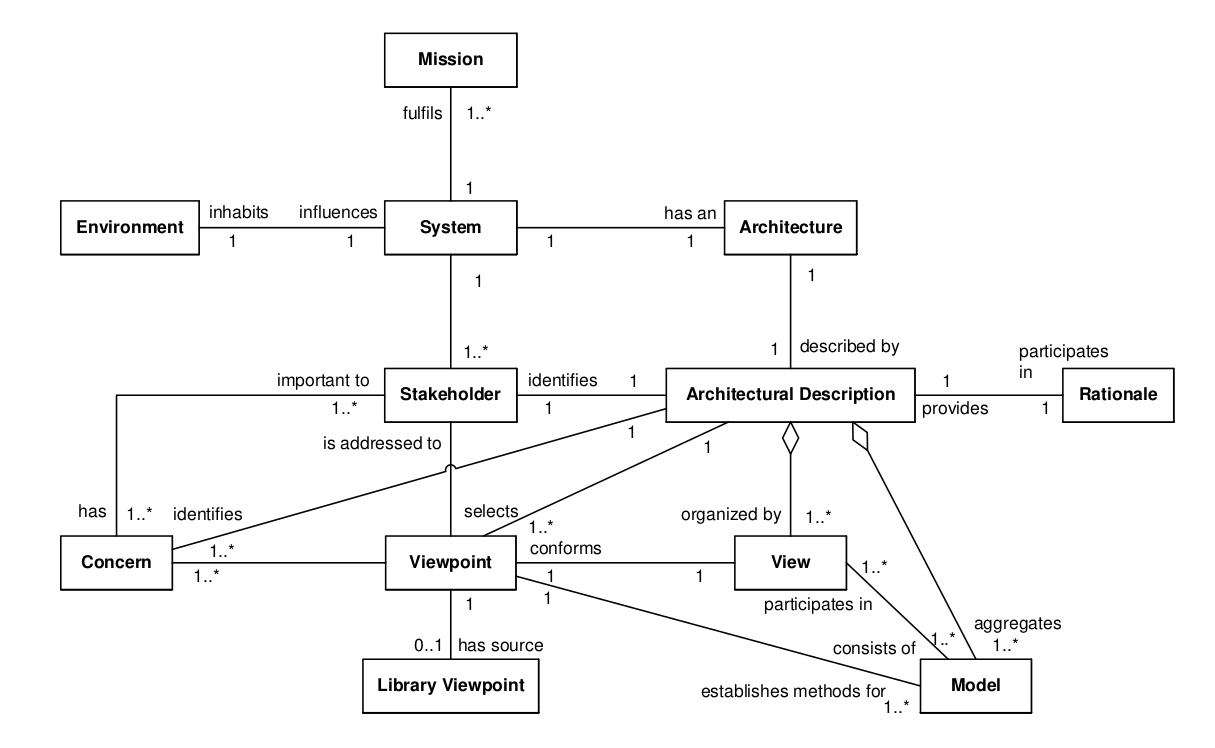
\includegraphics[width=.8\textwidth]{images/software_intensive_system_architecture.png}
  \caption{Architecture in Software Intensive Systems}\label{fig:software_intensive_system_architecture}
\end{figure}

\begin{itemize}
  \item The \textbf{system} is a collection of components which are organized to accomplish a function and has defined boundaries, consists of components and interfaces interacts with its environment through these interfaces and is defined by its static structure and dynamic behavior.
  \item The \textbf{environment} are the developmental, operational, political and other influences on the system.
  \item Every system has an \textbf{architecture} that can be described by an \textbf{architectural description}.
  \item \textbf{Stakeholders} are people that have an interest in the system which can have various roles regarding the architectural description.
  \item \textbf{Concerns} are interests which influence the system's development, its operation or any other aspect that is important to stakeholders.
  \item \textbf{Views} address one or more concerns of the system stakeholders.
  \item A \textbf{viewpoint} then describes a view and any associated modeling methods or analysis techniques by determining the languages for the architectural description
  \item \textbf{(System) models} provide abstractions in different ways.
    The object model describes the structure of the system, the functional model what the system's functions are and a dynamic model how the system reacts to external events.
\end{itemize}

\subsubsection{Modelling}
Models \textbf{reduce} the reality to a subpart of the original where irrelevant parts to the application are omitted which increases abstraction.
This reduction always has a \textbf{purpose} in mind which makes id adequate for a purpose or not and it is always possible to find a \textbf{mappging} between reality and the model.\\
The process of modelling can be divided in the following repeating sub-processes:
\begin{itemize}
  \item \textbf{Understanding} the application domain and its problems and possible solutions
  \item \textbf{Conceptualize} the part of the domain that is of relevance with the help of a concept language
  \item \textbf{Abstract} by outlining the main problems that have to be supported by the system on the basis of forgetful mappings.
  \item \textbf{Define} the main concepts/annotations used for the development of the model.
  \item \textbf{Construct} a model by organizing and linking ideas, judgements or concepts.
  \item \textbf{Evaluate} the model or parts of it considering pre-defined quality characteristics.
  \item \textbf{Refine} with iterative development to make the model more elaborated while maintaining its main structure.
\end{itemize}

\subsubsection{Modularity}
Modularity is the decomposition of a system into components to manage complexity by hiding unnecessary information to the outside world in these components.
This increases maintainability and reusability since the single components can be switched out or used elsewhere.
Also work can be easily distributed to the single components.\\
Functional decomposition decomposes the system regarding functions which implies that one has to understand the whole system to make a change possibly.
A better approach is modular decomposition where modules are the main concepts in a system.
This assumes we can find concepts in a new (greenfield engineering) or existing (reeingineering) software system  and that we can create a component-based interface on any system (interface engineering).\\
When looking at modules, we can either assume a black-box view where we only look at the possible input-output combinations and not the internals of the system or a whit-box view where the internals are regarded.

\subsubsection{Component-based Software Engineering (CBSE)}
CBSE is an approach to software development that relies on the reuse of software components which are a set of classes that can be considered a stand-alone service provider.
Components then interact with each other over published, clear defined and standardized interfaces and are integrated with the help of some middleware.\\
A software component has the following properties:
\begin{itemize}
  \item \textbf{Standardized}: Conformation to a standard component model
  \item \textbf{Independent}: Deployable without dependences to other components or if needed it should be stated in a ``requires'' interface specification.
  \item \textbf{Composable}: All interactions have to happen through the public interface
  \item \textbf{Deployable}: Ability to operate as stand-alone entity on a component platform that provides an implementation of the component. This usually means that binaries are provided so that no compilation is necessary before deployment.
  \item \textbf{Documented}: Syntax and also ideally semantics should be specified
\end{itemize}

Component interfaces are defined as shown in Figure~\ref{fig:component_interfaces}.\\
\begin{figure}[h]
  \centering
  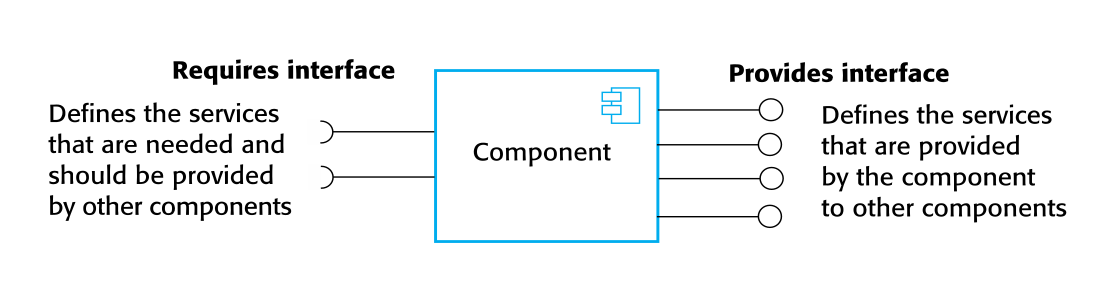
\includegraphics[width=.8\textwidth]{images/component_interfaces.png}
  \caption{Component Interfaces}\label{fig:component_interfaces}
\end{figure}

A component model is a definition of standards for component implementation, documentation and deployment as shown in Figure~\ref{fig:component_model}.
\begin{figure}[h]
  \centering
  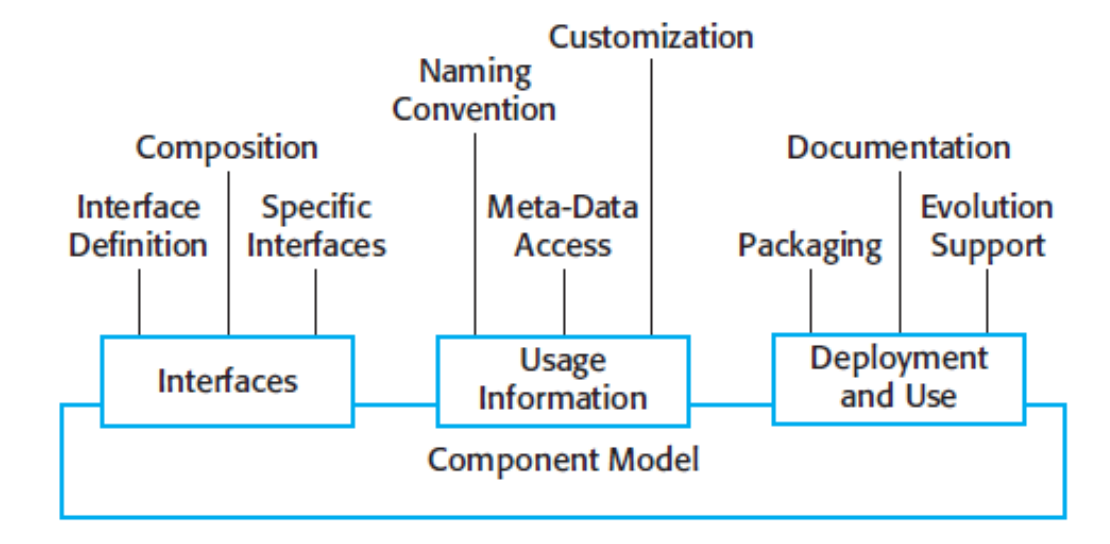
\includegraphics[width=.8\textwidth]{images/component_model.png}
  \caption{Component Model}\label{fig:component_model}
\end{figure}
It specifies how and in which language the interfaces should be defined and the elements which should be included (e.g.\ names, parameters,\ldots).
Furthermore naming conventions are defined for the usage of the component, e.g.\ URIs and meta-data is provided which gives information about interfaces, attributes and helps users to find out what services are provided and required.
Lastly the component model specifies how components should be packaged for deployment usually including all dependencies not specified in the ``required'' interface.\\

After the modelling of the components, they can be composed as shown in Figure~\ref{fig:component_composition}.
\newline

\begin{figure}[h]
  \centering
  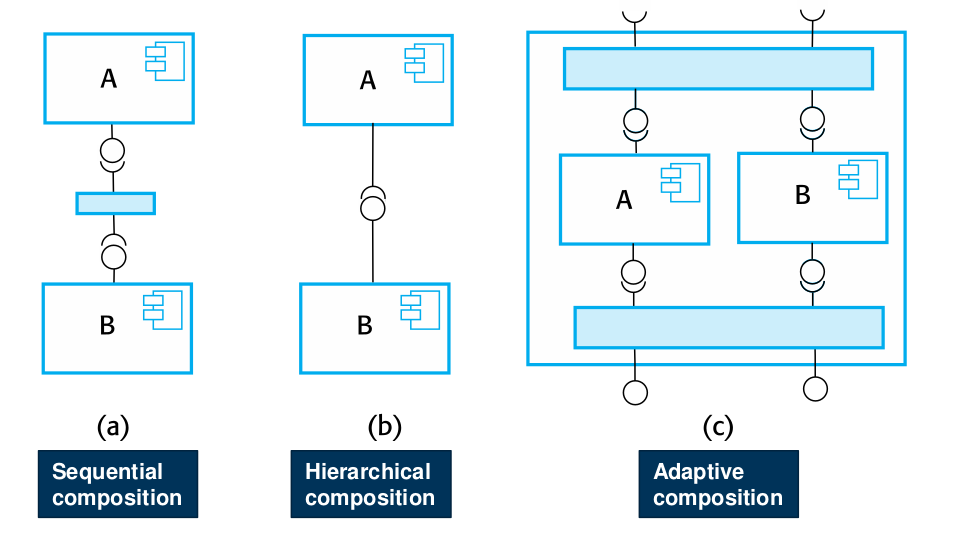
\includegraphics[width=.7\textwidth]{images/component_composition.png}
  \caption{Component Composition}\label{fig:component_composition}
\end{figure}

\begin{minipage}[t]{0.49\textwidth}
    \textbf{Pros}
    \begin{itemize}[topsep=0pt, itemsep=0pt]
        \item Independent components
        \item Component standards to facilitate integration
        \item Middleware to provide support for inter-operability
        \item Development process that is geared to reuse
    \end{itemize}
\end{minipage}
\begin{minipage}[t]{0.49\textwidth}
    \textbf{Cons}
    \begin{itemize}[topsep=0pt, itemsep=0pt]
        \item Component trustworthiness
        \item Component quality certification
        \item Emergent property prediction
        \item Requirements trade-offs (difficult analysis between features of two components)
    \end{itemize}
\end{minipage}

\subsubsection{Design by contract}
Design by contract presents a set of principles to produce dependable and robust object-oriented software.
Thereby a contract is an agreement between the client and the supplier.
Each party expects benefits from the contract and is prepared to incur some obligations to obtain them.
These benefits and obligations are documented in the contract where no obligations than the ones documented can be imposed to a party to obtain the benefits (no hidden clause rule).\\
The design principles design by contract proposes are
\begin{itemize}
  \item \textbf{Non-redundancy}: no tests of preconditions
  \item \textbf{Reasonable preconditions}: precondition is written in the documentation and can by justified according to that specification
  \item \textbf{Failure principle}: execution of rescue clauses to its and, not leading to a retry instruction, causes the current routine to fail.
  \item \textbf{Disciplined exception handling}: The two possible reactions to an exception are retrying or a failure/organized panic.
  \item \textbf{Exception simplicity} Simple rescue clauses that only bring the object back to a stable state, permitting a possible retry
\end{itemize}

\subsubsection{Dependency Structure Matrix (DSM)}
A DSM is a two-dimensional matrix representing the structural or functional interrelationships of objects, tasks or teams.
Each entry in the matrix indicates that the item on the corresponding column depends on the item on the corresponding row.\\
Partitioning on the matrix describes the transformation so that all dependencies are below the diagonal or within groups (interdependencies) and results in a block triangular matrix form.
To eliminate the groups/interdependencies, the corresponding rows and columns can be grouped to one (c.f.\ Figure~\ref{fig:dsm_grouping}).
\begin{figure}[h]
  \centering
  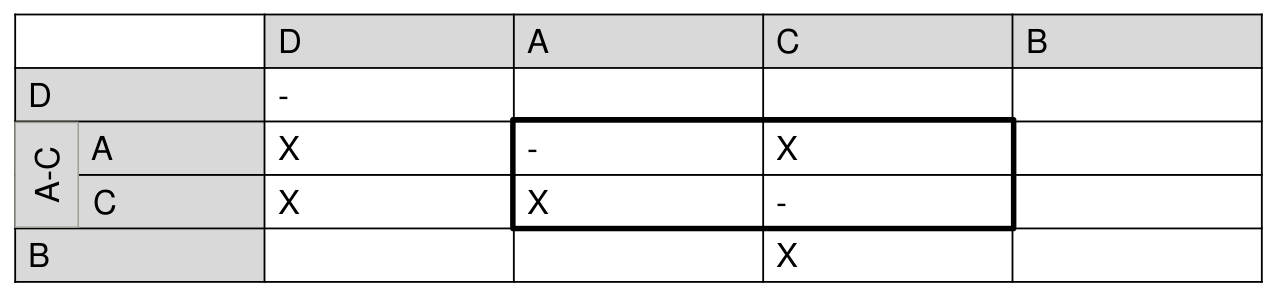
\includegraphics[width=.8\textwidth]{images/dsm_grouping.png}
  \caption{DSM Grouping}\label{fig:dsm_grouping}
\end{figure}

DSMs can be used to identify patterns an anti-patterns in software, c.f.\ Figure~\ref{fig:dsm_layered_pattern} and Figure~\ref{fig:dsm_propagator_anti_pattern}.

\begin{figure}
  \centering
  \begin{minipage}{0.49\textwidth}
    \centering
    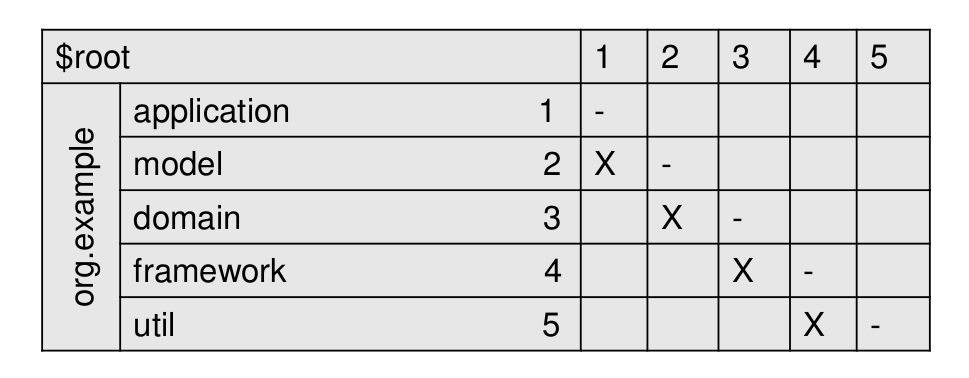
\includegraphics[width=\textwidth]{images/dsm_layered_pattern.png}
    \captionof{figure}{Layered Pattern in DSM}\label{fig:dsm_layered_pattern}
  \end{minipage}%
  \begin{minipage}{0.49\textwidth}
    \centering
    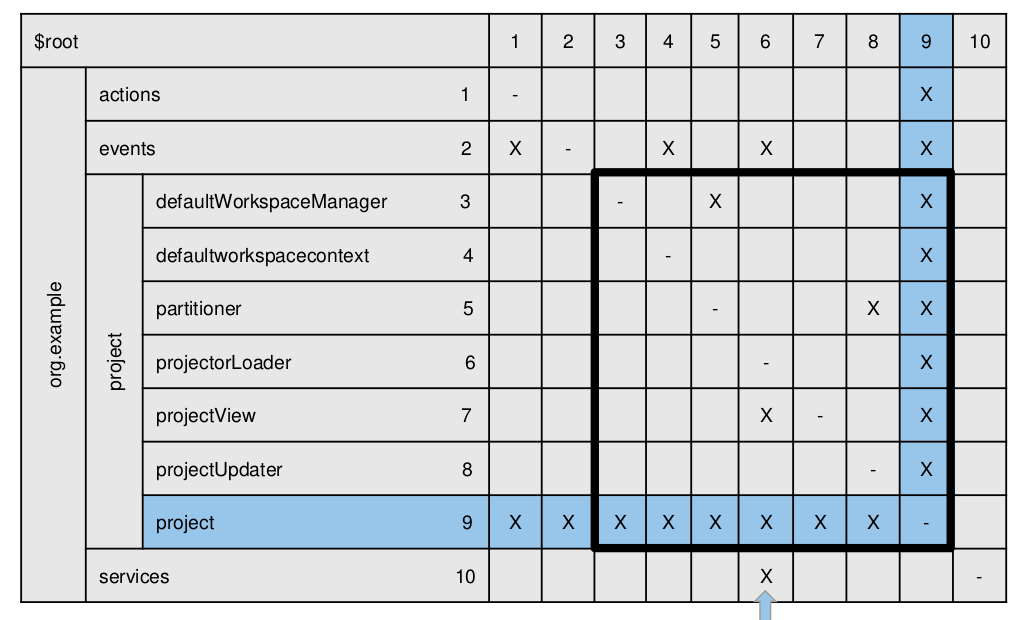
\includegraphics[width=\textwidth]{images/dsm_propagator_anti_pattern}
    \captionof{figure}{Propagator Anti-Pattern in DSM}\label{fig:dsm_propagator_anti_pattern}
  \end{minipage}
\end{figure}

\begin{minipage}[t]{0.49\textwidth}
    \textbf{Pros}
    \begin{itemize}[topsep=0pt, itemsep=0pt]
      \item Better scaling than box-and-line diagrams
      \item Better understanding of information flows
      \item Automatic partitioning algorithms
      \item Efficient cycle detection
      \item Integration of dependency rules
    \end{itemize}
\end{minipage}
\begin{minipage}[t]{0.49\textwidth}
    \textbf{Cons}
    \begin{itemize}[topsep=0pt, itemsep=0pt]
      \item Only as good as the knowledge that goes in (unknown dependencies might exist)
      \item less intuitive than a graph
    \end{itemize}
\end{minipage}

\subsubsection{Guidelines for Modular Design}
\paragraph{Low Coupling and High Cohesion}
We denote the structure of a system as $S = (C,I,CON)$ where C are the components, $env \in C$ the environment, I the interfaces and $CON \subseteq I x I$ is the connection between interfaces.
Figure~\ref{fig:system_structure_notation} shows the notation and possible relationships between components.
\begin{figure}[h]
  \centering
  \begin{subfigure}{.3\textwidth}
    \centering
    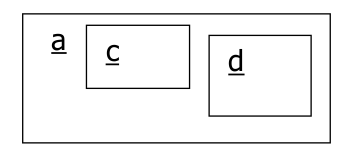
\includegraphics[width=\textwidth]{images/component_parent_relationship.png}
    \caption{Parent relationship\\ $parent(c) = parent(d) = a$\\ $parent(a) = env$}
  \end{subfigure}
  \hspace{.03\textwidth}
  \begin{subfigure}{.3\textwidth}
    \centering
    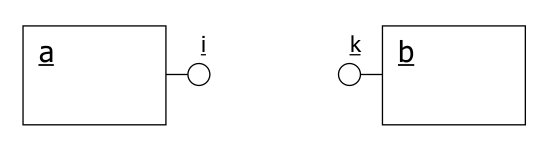
\includegraphics[width=\textwidth]{images/component_interface_relationship.png}
    \caption{Interface-Component Relationship\\ $assigned(i) = a$\\ $assigned(k) = b$}
  \end{subfigure}
  \hspace{.03\textwidth}
  \begin{subfigure}{.3\textwidth}
    \centering
    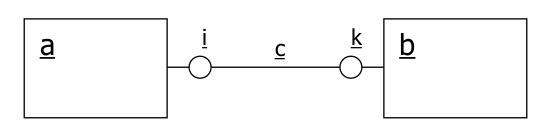
\includegraphics[width=\textwidth]{images/component_connection.png}
    \caption{Connection between Interfaces\\ $connected(c) = (i,k)$}
  \end{subfigure}
  \caption{System Structure Notation}\label{fig:system_structure_notation}
\end{figure}

We then define \textbf{coupling} as the normalized number of connections between components at the same hierarchical level 
\begin{equation*}
  coupling(s) = \frac{|\{con \in s.CON| \exists s,I: con = connected(i,j) \wedge parent(assigned(i)) = parent(assigned(i))\}|}{|s.C|}.
\end{equation*}
The goal is to make coupling as low as possible.

We can define different classes of coupling, in the following listed in decreasing amount of coupling order:
\begin{itemize}
  \item \textbf{Content Coupling}: One component changes another component's data or when control is passed from one component to the middle of another.
  \item \textbf{Common Coupling}: Two components share data which shows a lack of clear responsibility and reduces readability, maintainability and reusability
  \item \textbf{External Coupling}: Components communicate through an external medium such as a file, device interface, protocol or data format.
  \item \textbf{Control Coupling}: One Component directs exaction of another component by passing the necessary control information. This approach can be good if parameters allows factoring and reuse of functionality or bad if parameters indicate completely different behavior or components are not independent.
  \item \textbf{Stamp Coupling}: Complete data structures are passed from one component to another.
  \item \textbf{Data Coupling}: Component passes data (not data structures) to another component.
\end{itemize}

\textbf{Cohesion} is defined as how closely related different responsibilities of a component are. The goal is to make cohesion as high as possible.\\
Like for coupling, we can again define types of cohesion, also in decreasing order:
\begin{itemize}
  \item \textbf{Functional Cohesion}: Every essential element to a computation is contained in the component so that a single input is transformed to a single output. Ideal kind of cohesion in that it maximizes reusability, testability, understandability, learnability, extensibility and maintainability.
  \item \textbf{Sequential Cohesion}: The output of one component is the input of another and data flows between parts. Quite good kind of cohesion.
  \item \textbf{Communicational Cohesion}: Elements operate on the same data
  \item \textbf{Procedural Cohesion}: Elements are related only to ensure a particular order of execution. Actions are weakly connected and unlikely to be reusable
  \item \textbf{Temporal Cohesion}: Elements are independent but are activated around the same point in time. Code is spread out which results in bad maintainability and reusability
  \item \textbf{Logical Cohesion}: Elements are logically related, not functional
  \item \textbf{Coincidental Cohesion}: Elements have no significant relation to each other (worst kind).
\end{itemize}

\paragraph{Single Responsibility Principle}
Every class should only have one responsibility, if there are multiple split the class.
A guideline for this is ``there should never be more than one reason to change a class''.

\paragraph{Separation of Concerns}
Separate features to different components which encapsulate a semantic concern what helps humans to handle complexity (only able to hold around 7 things in mind).
This also enables components to be easily replaced.
Modules therefore designed with the \textbf{open/closed principle} in mind.
This means that a module is open for extension but closed for modification so that the behavior cannot be changed but only extended and thus no unexpected effects will arise.

\paragraph{Liskov Substitution Principle (LSP)}
\begin{chapquote}{Barbara Liskov. (1987)}
    Let $q(x)$ be a property provable about objects x of type T. Then $q(y)$ should
be provable for objects y of type S where S is a subtype of T.
\end{chapquote}
This means child classes should never violate the invariants of the base class or remove some of its behavior.

\paragraph{Interface-Segregation Principle}
Prefer small, cohesive interfaces over big ones.

\paragraph{Anticipate change}
Build components in a way that minimizes effort for potential future changes by finding a compromise between generality and specificity.
A good guideline here is the principle of low coupling and high cohesion.
It is easy to overdo it though, since reusability is oftentimes very difficult.

\paragraph{Do not Repeat Yourself}
Every piece of knowledge (and functionality) must have a single, unambiguous, authoritative representation within a system.
This dramatically improves maintainability.\\
Duplication can either be imposed (developers have no choice due to environment), inadvertent (duplication not realized by devs), due to impatience or lazyness or due to inter-developer communication or the lack thereof.

\subsubsection{Architecture and External Quality}
When introducing a high degree of modularity we influence internal quality by increasing maintainability and reusability.
Testability might be increased or decreased depending on the system though.
External quality might suffer also by introducing to many layers or indirections
which decreases performance and also security might suffer by introducing large attack surfaces.\\

\subsection{Antipatterns}
Antipatterns are commonly occurring solutions to a problem that generates decidedly negative consequences.
They define an industry vocabulary for common defective processes and implementations within organizations.
Antipatterns can concern software development and software architecture.\\
The reasons for these mistakes are called the 7 deadly sins:
\begin{itemize}
  \item Haste
  \item Apathy (not caring)
  \item Narrow-Mindedness (not applying common solutions)
  \item Sloth (solutions based on easy answers)
  \item Avarice (excessive complexity)
  \item Ignorance
  \item Pride
\end{itemize}

Common antipatterns are:
\begin{itemize}
  \item The blob: A ``god class'' that does everything typically caused by the lack of an architecture or the enforcement thereof, too limited intervention or by the specification of the requirements. 
  \item Functional decomposition: Modules are based on functionality instead of semantic parts from the view of the user. It is typically caused by a lack of object-oriented understanding, the lack of architecture enforcement and sometimes due to badly specified requirements
  \item Auto-generated stovepipe: Trying to use the same interfaces of an existing system for a distributed one.
  \item Golden Hammer: Using the same tools for everything
  \item Design by committee: A complex software design is the product of a committee process of too many people. The design is too complex to realize and test due to excessive complexity, ambiguities, over constraint and other specification defects.
\end{itemize}

\subsection{Reuse}
When developing software, it is usually advisable to ``invent the wheel twice''.
Therefor components should be designed with some principles in mind to support reuse:
\begin{itemize}
  \item Modularity to extract and insert modules
  \item Loose coupling high cohesion also to extract modules
  \item Information hiding for plug and play usage
  \item Separation of concerns to be able to tell the responsibilities of a component
\end{itemize}
There are some pitfalls when trying to write reusable components though.
Either technical issues like the reuse is only done at code level which has a very limited scope and is often done unsystematically  or inconsistent or incomplete component specifications reusability or organizational reasons like the lack of planning, motivation or component marketplaces can hinder the development of reusable software.
Also everytime a trade-off between flexibility and stability has to be met so that enough flexibility that reuse is feasible and enough stability to generate benefits is given.\\
Reusable components can either be a side product of development (opportunistic or ad-hoc reuse) or be planned (planned or structured reuse).
Ad-hoc reuse usually dues not scale due the lack of infrastructure to maintain components like search, evaluation, adaption or integration services.
So the better approach is structured reuse where essential functionality is parameterized so that it can easily be customized usually during deployment.\\

\subsubsection{Variability}
Variability can either be visible to the user (external variability) or hidden from them (internal variability).
It is supported by the concept of managed variability which implies defining variability, managing variable artifacts, supporting activities concerned with resolving variability and collecting, storing and managing trace information necessary to fulfill these tasks.
The time when variabilities are resolved is called binding time.\\
Defining variability can be done as an integral part of development artifacts, which increases their complexity though, or in a separate model.

\paragraph{Orthogonal Variability}
An orthogonal variability model is a model that defines the variability of a software product line. It relates the variability defined to other software development models such as feature model, use case models, design models, component models, and test models.\\

On requirement level, variability is modeled as feature diagram where parts can be mandatory or optional and have interdependencies.
A variation point is defined as a representation of a variability subject and a variant then is a representation of a variability point.
Figure~\ref{fig:feature_diagram} shows an example of a feature diagram.\\
\begin{figure}[h]
  \centering
  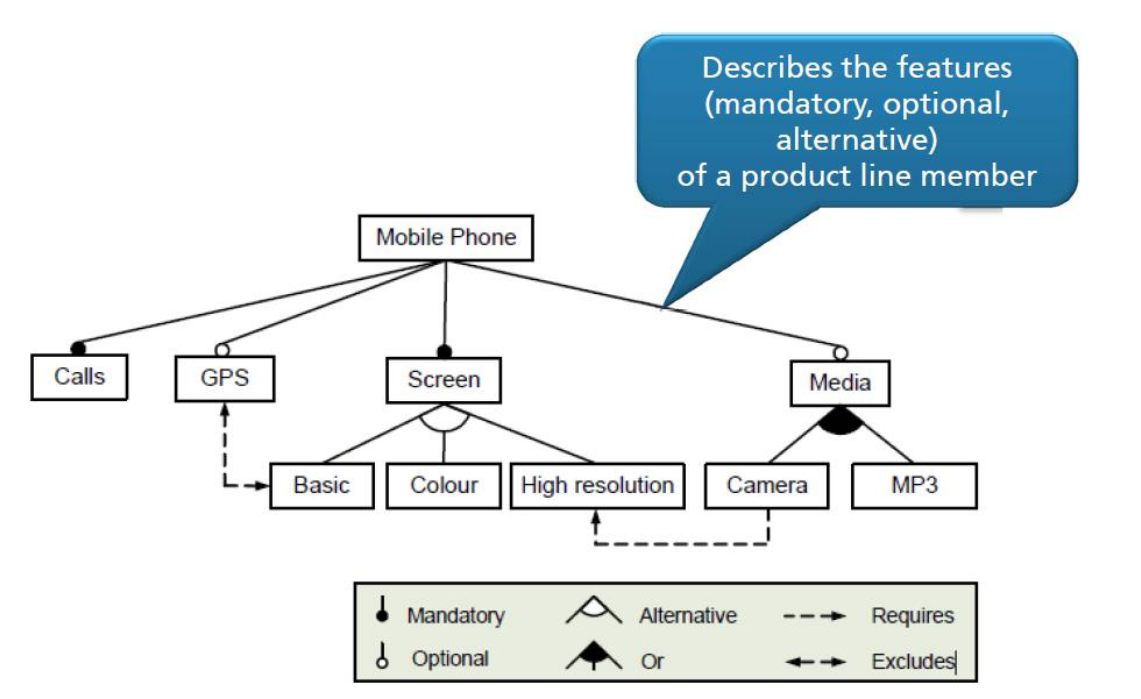
\includegraphics[width=.8\textwidth]{images/feature_diagram.png}
  \caption{Feature Diagram}\label{fig:feature_diagram}
\end{figure}

On code level, variety can be supported with conditional compilation, polymorphism, frame technology or aspect-oriented programming.

\subsubsection{Product Line Engineering (PLE)}
A software product line is a set of applications with a common architecture and shared components, with each application specialized to reflect different requirements.
Specialization can take place in several domains including platform, environment, functions and processes.\\
PLE then is the process of developing a product line with a heavy focus on reusability by separating development into \textbf{family engineering} and \textbf{application engineering}.
Figure~\ref{fig:product_line_engineering} shows an illustration of this process.
\begin{figure}[h]
  \centering
  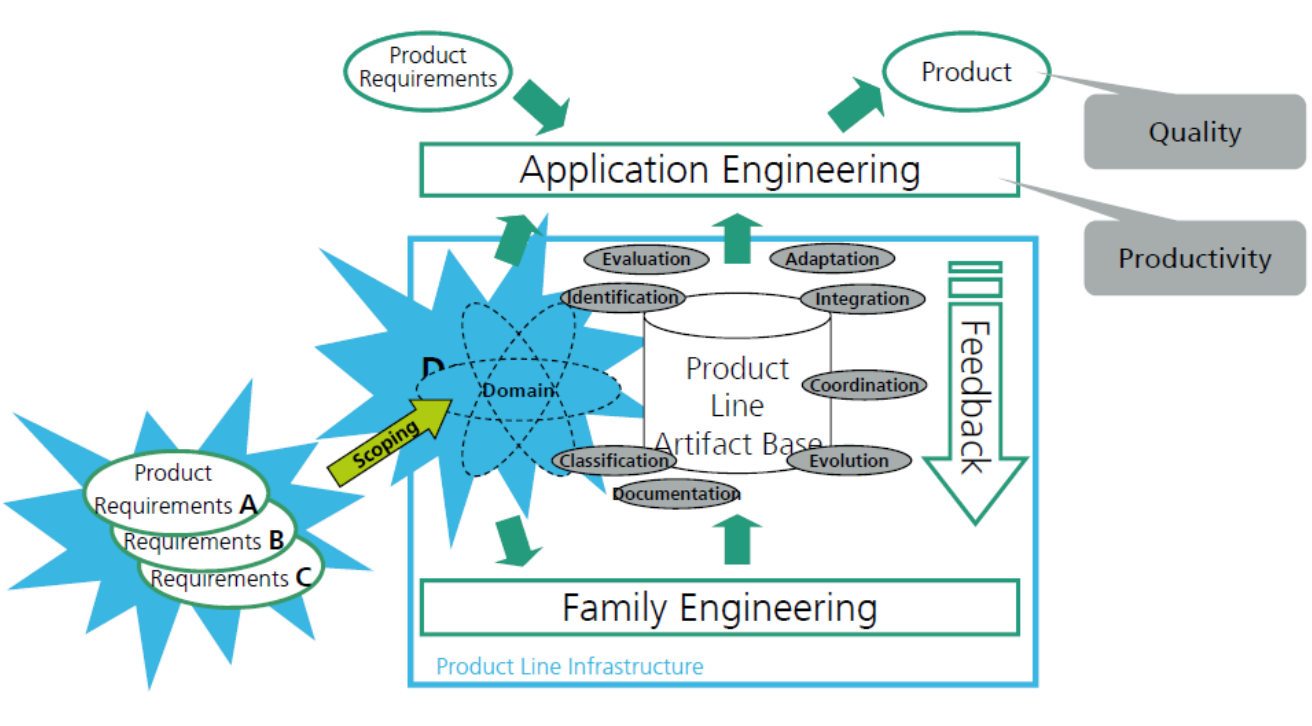
\includegraphics[width=.7\textwidth]{images/product_line_engineering.png}
  \caption{Product Line Engineering}\label{fig:product_line_engineering}
\end{figure}
In family or domain engineering product commonalities and variabilities are identified and reusable (product line) artifacts are developed.
An essential part of this is the scoping of the product line by defining sharp boundaries based on most of the concrete product requirements (all is not economical most of the time).
Important aspects of this are which products will be in the line, which domains to consider, which features are required and which assets are in the line.
These base artifacts cover variability as well as commonalities of the PL and are stored in the \textbf{product line artifact base}.
During the application engineering process their variabilities then are instantiated according to the specific product requirements and thus individual products are developed.\\

\begin{minipage}[t]{0.49\textwidth}
    \textbf{Pros of well-done PLE}
    \begin{itemize}[topsep=0pt, itemsep=0pt]
        \item Reduces development costs
        \item Increases quality
        \item Decreases time-to-market
        \item Better understanding of the domain
        \item Structured reuse possible
    \end{itemize}
\end{minipage}
\begin{minipage}[t]{0.49\textwidth}
    \textbf{Cons}
    \begin{itemize}[topsep=0pt, itemsep=0pt]
        \item High up-front invenstments
        \item Strong domain knowledge and therefore experts necessary
        \item May result in a badly scoped domain what leads to unwanted assets
        \item Limited success in reality
    \end{itemize}
\end{minipage}

\subsubsection{Reference Architectures and Frameworks}
\paragraph{Software Frameworks}
A framework is a set of classes that embodies an abstract design for solutions to a family of related problems, and supports reuse at a larger granularity than classes.
Frameworks support design reuse by providing a skeleton architecture for the application as well as the reuse of specific classes and are language specific.
Applications using a framework extend generic classes of the framework in so called extension points or hot-spots.\\
The main difference to a library is the call hierarchy.
Frameworks call the application specific classes whereas when using a library the application calls the library code.
Also frameworks usually already provide a semi-complete application whereas libraries are only pluggable parts of it.

\paragraph{Reference Architectures}
A Reference architecture is an abstract software architecture for a specific application area. It defines structures and types of software elements, and their interactions and responsibilities. The defined structures are applicable for all systems of a domain.
There are three different types of reference architectures described in Figure~\ref{fig:reference_architectures}.
\begin{figure}[h]
  \centering
  \begin{tabular}{|p{.225\textwidth}|p{.225\textwidth}|p{.225\textwidth}|p{.225\textwidth}|}
    \hline
    & Functional & Logical & Technical\\
    \hline
    Phase of the development process & Requirements analysis & Conceptual design & Detailed design, Implementation\\
    \hline
    Provides a basis for & Functional specification, planning of subsystems & Logical architecture, planning of the implementation & Detailed architecture, implementation, deployment\\
    \hline
    Elements & Functional areas as units of functionality & Components as units of design and implementation & Components as units of implementation and deployment\\
    \hline
    Stakeholder & User, manager, project leaders & Project leaders, architects, developers & Architects, developer, maintenance staff\\
    \hline
    Architectural overview & Functional areas, data flow & Components, layers to be implemented & Technical components, layers which can be deployed\\
    \hline
    Textures (structures, principles and design concepts which occur often) & - & Design rule, may be expressed as a design pattern & Design rule, design pattern, code template\\
    \hline
    Reference interfaces & Named interfaces, if any & Named interfaces; defined in an implementation neutral definition language (e.g., IDL), if necessary & Defined in the programming language used\\
    \hline
    Infrastructure & - & Basic properties & Exactly defined\\
    \hline
  \end{tabular}
  \caption{Types and Elements of a reference architecture}\label{fig:reference_architectures}
\end{figure}
